Para visualizar los resultados ejecutados en otro equipo, se debe realizar “make run” desde:
\begin{itemize}
    \item \texttt{../code/matrix\_multiplication} -> ejecutar multiplicación de matrices.
    \item \texttt{../code/sorting} -> ejecutar ordenamiento.
\end{itemize}

Al terminar la ejecución, los resultados estarán en:
\begin{itemize}
    \item \texttt{../code/matrix\_multiplication/data/matrix\_output} -> contiene carpetas (naive y strassen) con los resultados de las multiplicaciones en archivos de texto.
    \item \texttt{../code/sorting/data/array\_output} -> contiene carpetas (mergesort, quicksort, selectionsort y sort) con los resultados de los ordenamientos en archivos de texto.
\end{itemize}

Además, se pueden revisar los tiempos y el uso de memoria en:
\begin{itemize}
    \item \texttt{../code/matrix\_multiplication/data/measurements} -> archivos de texto para cada implementación de multiplicación de matrices.
    \item \texttt{../code/sorting/data/measurements} -> archivos de texto para cada implementación de ordenamiento.
\end{itemize}

Cabe destacar que la ejecución de estos algoritmos puede arrojar resultados distintos en cada implementación, ya que se generan nuevos datasets tanto para la multiplicación de matrices como para el ordenamiento. Además, el hardware del equipo en que se ejecuten los programas influye significativamente en el desempeño en términos de tiempo y memoria. No obstante, la tendencia general de los resultados no debería verse alterada, permitiendo replicar el análisis presentado en este informe sin modificar las conclusiones teóricas.

\newpage
Para el análisis de los algoritmos de ordenamiento, se realizaron pruebas utilizando distintos datasets, lo que permitió ampliar el estudio sobre su comportamiento. Inicialmente, como se muestra en la \autoref{fig:Figura1}, los tiempos de ejecución fueron similares hasta datasets de tamaño 100.000, donde comienza a evidenciarse una diferencia considerable en el tiempo requerido por selectionsort, y una leve diferencia respecto a quicksort.\\
Al aumentar las pruebas a datasets con 10.000.000 de elementos, se observa claramente el desempeño de mergesort y sort. Es importante señalar que no se realizaron pruebas con quicksort en estos últimos datasets debido a errores de segmentation fault en cada archivo, ni con selectionsort, dado que su ejecución supera las 5 horas de ejecución por archivo.\\


\begin{figure}[H]
    \centering
    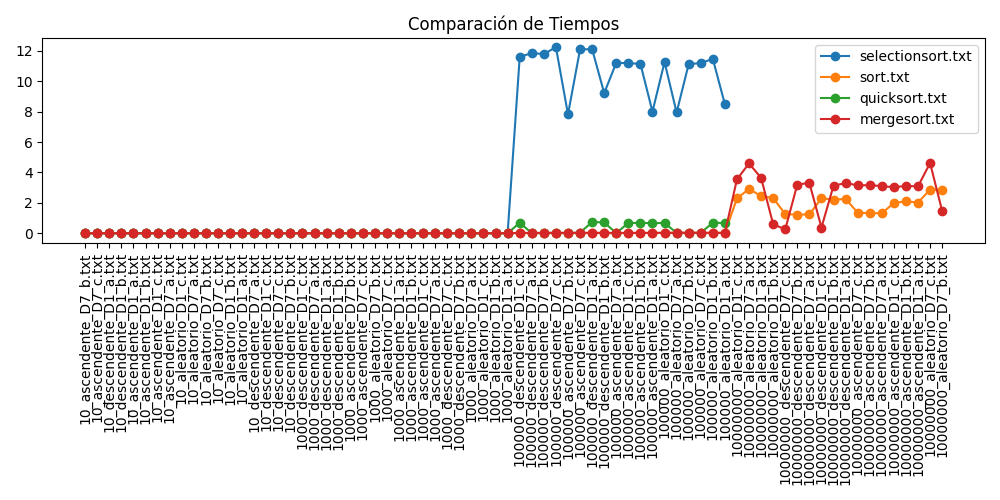
\includegraphics[width=\textwidth]{../code/sorting/data/plots/Grafico_tiempos.png}
    \caption{Tiempo en segundos empleado por cada ordenamiento}
    \label{fig:Figura1}
\end{figure}

\newpage
El uso de memoria para los archivos fue similar en todos los casos analizados hasta los datasets de tamaño 100.000 como se puede observar en la \autoref{fig:Figura2}. No obstante, no fue posible comparar el uso de memoria de quicksort y selectionsort en datasets de 10.000.000 elementos, ya que no se realizaron dichas pruebas. En particular, quicksort presentó errores de segmentation fault en todas las ejecuciones con estos últimos datasets, debido a que el uso de memoria superó el límite de stack asignado por el sistema. Esta situación se explica por la gran cantidad de llamadas recursivas provocadas por una mala elección de pivotes, generando una gran profundidad en la recursión.\\

\begin{figure}[H]
    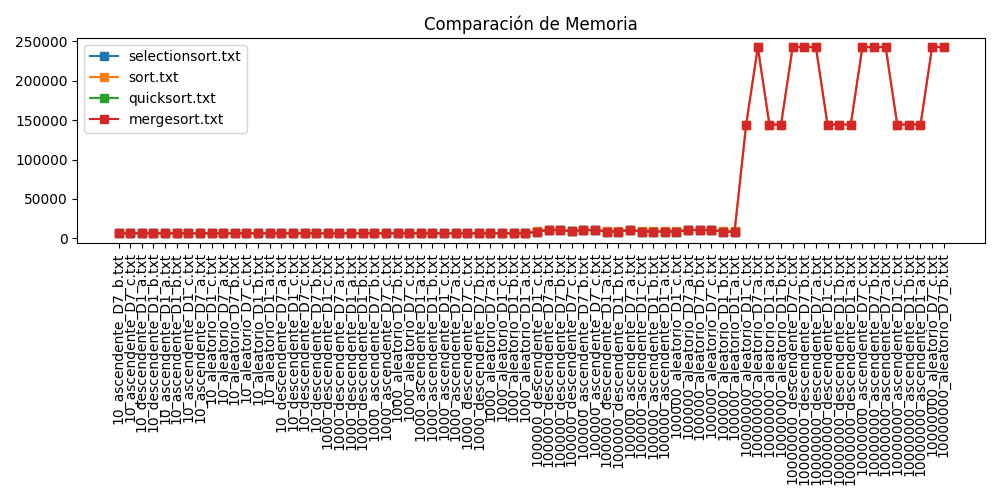
\includegraphics[width=\textwidth]{../code/sorting/data/plots/Grafico_memoria.png}
    \caption{Memoria en kilobytes utilizada por cada ordenamiento}
    \label{fig:Figura2}
\end{figure}

\newpage
Para el análisis de los algoritmos de multiplicación de matrices se realizaron pruebas utilizando distintos datasets, lo que permitió ampliar el estudio sobre su comportamiento. Como se observa en la \autoref{fig:Figura3}, los tiempos de ejecución fueron similares para ambas implementaciones en los primeros tamaños de matrices. Sin embargo, a partir de matrices de tamaño 1024×1024, el algoritmo de Strassen aumentó significativamente el tiempo de ejecución, lo cual resulta curioso considerando que, teóricamente, su orden de complejidad es menor que el de naive. Esto se explica porque Strassen realiza muchas operaciones costosas que no son eficientes para datasets relativamente pequeños. Se proyecta que los resultados favorables para Strassen se observarán en matrices de tamaño aún mayor, donde naive incremente considerablemente sus tiempos de ejecución.\\

\begin{figure}[H]
    \centering
    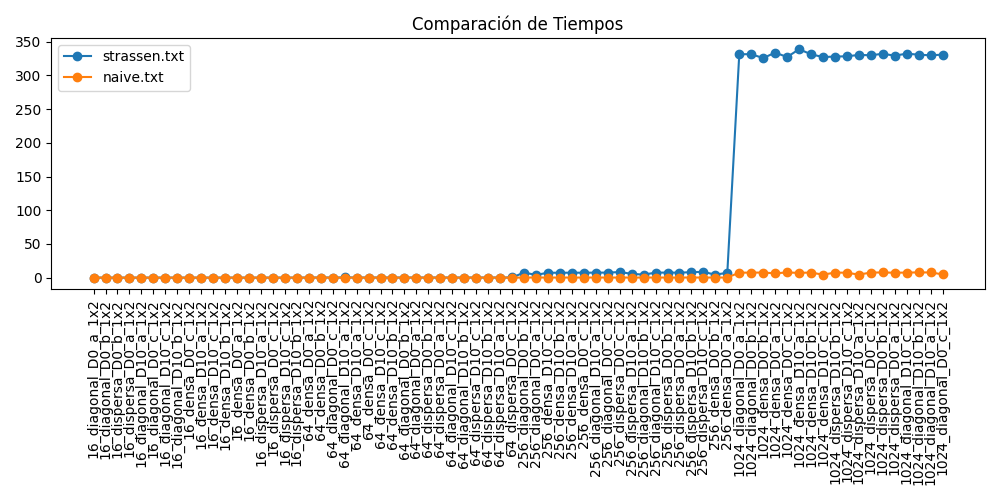
\includegraphics[width=\textwidth]{../code/matrix_multiplication/data/plots/Grafico_tiempos.png}
    \caption{Tiempo en segundos empleado por cada multiplicación}
    \label{fig:Figura3}
\end{figure}

\newpage
El uso de memoria para los archivos fue similar en todos los casos analizados, como se observa en la \autoref{fig:Figura4}. Se observa una leve diferencia en el consumo de memoria por parte de strassen, se debe a las operaciones internas adicionales que realiza en comparación con naive. No obstante, esta diferencia podría incrementar a medida que aumente el tamaño de los datasets.\\

\begin{figure}[H]
    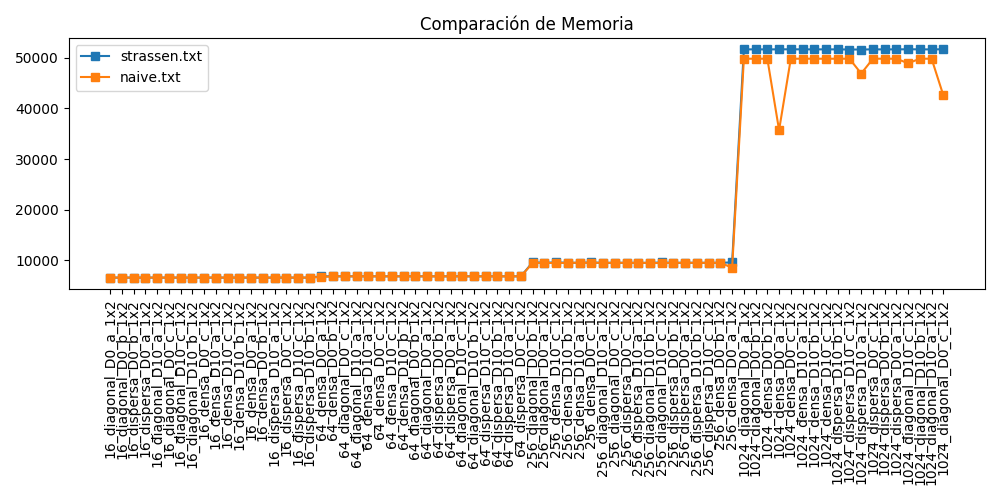
\includegraphics[width=\textwidth]{../code/matrix_multiplication/data/plots/Grafico_memoria.png}
    \caption{Memoria en kulobytes utilizada por cada multiplicación}
    \label{fig:Figura4}
\end{figure}